\documentclass{article}
\usepackage{amsmath, amssymb, cite, algorithmic, url, braket}
\usepackage{graphicx}
\usepackage{pythonhighlight}
\usepackage[margin=1.5cm]{geometry}
\usepackage[title]{appendix}
\usepackage{listings}

\graphicspath{{../pic/}}
\lstset{
language=[ANSI]{C},
showtabs=true,
tab=,
tabsize=2,
basicstyle=\ttfamily\footnotesize,%\setstretch{.5},
stringstyle=\color{stringcolour},
showstringspaces=false,
alsoletter={1234567890},
otherkeywords={\%, \}, \{, \&, \|},
keywordstyle=\color{keywordcolour}\bfseries,
upquote=true,
morecomment=[s]{/*}{*/},
commentstyle=\color{commentcolour}\slshape,
literate=*%
{=}{{\literatecolour=}}{1}%
{-}{{\literatecolour-}}{1}%
{+}{{\literatecolour+}}{1}%
{*}{{\literatecolour*}}{1}%
{!}{{\literatecolour!}}{1}%
{[}{{\literatecolour[}}{1}%
{]}{{\literatecolour]}}{1}%
{<}{{\literatecolour<}}{1}%
{>}{{\literatecolour>}}{1}%
% {>>>}{\pythonprompt}{3}%
,%
frame=trbl,
rulecolor=\color{black!40},
backgroundcolor=\color{white},
breakindent=.5\textwidth,frame=single,breaklines=true
}

\begin{document}
\title{DSP Homework 01}
\author{Xu, Minhuan}
\maketitle
\tableofcontents

\begin{abstract}
    In this article, I solved 4 problems assigned. Answers lie in different sections respectively and the codes mentioned are in the 'code listing' section in the last part of this article.
\end{abstract}

\section{Problem 1}
\subsection{Problem Description}

Write a summary of this week’s video(s) and your further thought on the content.

\subsection{Summary and My Thoughts}
\subsubsection{Spending Money on others}

This is a very thought-provoking video, the talker tells us that one will acquire more happiness when he or her spends money on others, no matter how much the money is, than those who spend the same amount of money on themselves.

What impressed me most is that the test assuming that you give us a certain amount of money to see whether we will spend it on others. I remember I choose to spend the money on myself, which is for me a half-joke, and after thinking carefully, I believe that spending money on others is more pleasing on most occasions.

\subsubsection{Coffee Machine}

The creator of this video wants to have a cup of hot coffee just after he getting up, but the coffee machine can't run automatically. Luckily, he's an engineer, so he wants to control the machine remotely.

He has an esp32 which can work as the machine controller and the local server of http, but this chip is working on 5 Volts, and the coffee machine is working on over 200 Volts. So, a relay is essential, this little thing allows a very low voltage to control the on-off of a high-voltage circuit.

After coding and writing the program to the chip, his smartphone can perfectly send request to the local server to start/stop the machine (Answer can also be received). That's pretty cool.

For us, it is meaningful to care about things like this, because these little improvement of way of life is what alternatively lead to our tech development.

\section{Problem 2}

\subsection{Problem Description}

Write a mini-article on the human brain or nervous system and how marvelous it is (at signal processing, for example).
\subsection{Preface}

All I want to talk about is how the nervous system is to send the physical senses to out brain and what the reflex arc (especially conditioned reflex) means.

\subsection{How to SENSE}

We human have nerve cells called receptor near the surface of our body, these cells enable us to feel things outside. When the receptors stimulated by force or changes of the temperature, ion channels on cell membrane surface open, so the changes of inner and outer membrane voltage difference of nerve cells, resulting in the bioelectric current. This is how the touch and temperature be translated into electric signal. Moreover, the electrical signal conducts between the nerve cells through chemicals emitted by the synapse of nerve cells.\cite{receptor} This point is rather easy and mentioned in our textbook in high school.

\subsection{What is REFLEX}

After the receptor cell inside ourselves is stimulated by the outside, the ion channel on the surface of the cell membrane opens, which changes the voltage of the inner and outer membranes of nerve cells. Before stimulation, the potential difference between the inner and outer membranes is positive outside and negative inside, and after opening, it becomes negative outside and positive inside. This section of negative outside and positive inside is transmitted along the nerve cells, which becomes a biological current Where nerve cells and nerve cells come into contact, current is transmitted to the next cell through synapses

All I want to talk about is how the nervous system is to send the physical senses to out brain and what the reflex (especially conditioned reflex) means.

First, we human have nerve cells called receptor near the surface of our body, these cells enable us to feel things outside. When the receptors stimulated by force or changes of the temperature, ion channels on cell membrane surface open, so the changes of inner and outer membrane voltage difference of nerve cells, resulting in the bioelectric current. This is how the touch and temperature be translated into electric signal. Moreover, the electrical signal conducts between the nerve cells through chemicals emitted by the synapse of nerve cells.  This point is rather easy and mentioned in our textbook in high school.

Second, with signals above passing between cells inside our body, the nervous system can make very complicated actions become true. The reflex means the regular response of humans and animals to stimuli, it is the basic way for the nervous system to regulate various functional activities of the body.\cite{reflex_arc} The reflex can be divided into two kinds of conditional reflex and unconditioned reflex. We can distinguish the two by judging whether the reflex is inborn or can be acquired, the key to establishing conditional reflex is repeat (or exercise), just like the examination of Pavlov's dog. For example, people's learning process is the process of establishing conditioned reflexes. So, apparently, we should put more attention in conditional reflex, and if one want to gain solid knowledge, you should always review and strengthen what you learn.

\section{Problem 3}

\subsection{Problem Description}
Write a program to compute the expression composed of rational numbers and $+,\; -,\; * \;(\times), \; / \;(\div)$ which is split by space.

\subsection{Solution}
The first idea in my mind is to write a python script with the help of the module 'sympy', but it is too boring. So, I changed my goal to write a C script, and the work was hard for a long blank period. As a result, I again changed my language into python and write a solution without importing any external module.

After spending some time, I complete all of the scripts, and now I have 3 in my disk. I'll list the features of them below.

\begin{enumerate}
    \item python with sympy
            It is the shortest of the three, but the most other's codes are used. It can really deal with almost rational numbers.
    \item python without sympy
            It has the middle length thanks for python. What's more, it is easy to write. Its acceptable input is narrowed to fractions.I split both of the rational numbers into two integers, and calculate them following the rule of fraction, and print them in the required manner.
    \item C
            It is the longest of the three, but it is difficult to realize the function required because it is closer to the hardware. It can only process the expression composed of positive fractions with only two digits on its denominator and numerator. The idea of this code is mostly the same as the python one, but the realization is quite different.
\end{enumerate}

\section{Problem 4}
\subsection{Problem Description}
For your smart phone, laptop or desktop computer screen:
\begin{enumerate}
    \item[(a)] Find out its model and resolution.
    \item[{b}] Find out its color pixel pattern.
    \item[{c}] Propose a better color pixel arrangement pattern.
\end{enumerate}

\subsection{Answers}
The machines I investigated are my pad whose model is 'XiaoMi pad 5 pro' and my laptop whose model is 'Lenovo XiaoXin 13 pro 2020'.
\subsubsection{My pad}
\begin{enumerate}
    \item Model: a certain model produced by TCL CSOT; Solution: $2560\times1600$
    \item Standard RGB
    \item Today's arrangements for color pixel are pretty good, considering the authenticity, brightness, accuracy and lifespan. However, for me, the most important is authenticity and lifespan, so I will add some space into the pixels arranged by standard RGB to guarantee these two factors.
\end{enumerate}

I sprinkled some water on my pad, and some little water drops work as the magnifier. I pictured the pattern and compared it with the patterns and their name, coming out that my pad's color pixel pattern is Standard RGB.

\begin{figure}[htbp]
    \centering
    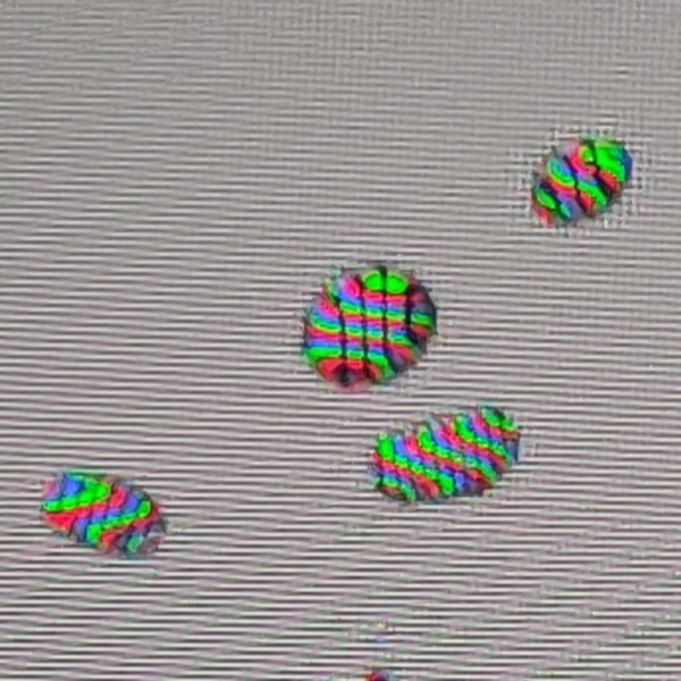
\includegraphics[keepaspectratio,width=150pt]{pixel.jpg}
    \caption{Color Pixel Pattern of My Pad}
\end{figure}

Then, I tried my best to find out the model of my pad's screen. I searched in the system config, only to find the resolution of my screen, so I searched on the internet and failed until I met another post which told me a new method of exporting the bugreport which can tell which company produced the screen. I tried this method, but there's no more information except the producer.

\subsubsection{My Laptop}
After investigating my pad, I am interest in my laptop again, so I do the work again.
\begin{enumerate}
    \item Model: CSO076D produced by TCL CSOT; Solution: $2560\times1600$.
    \item Standard RGB
\end{enumerate}

What makes me surprise is this screen has almost the same parameters. I will show the picture of the color pixel pattern below.

\begin{figure}[htbp]
    \centering
    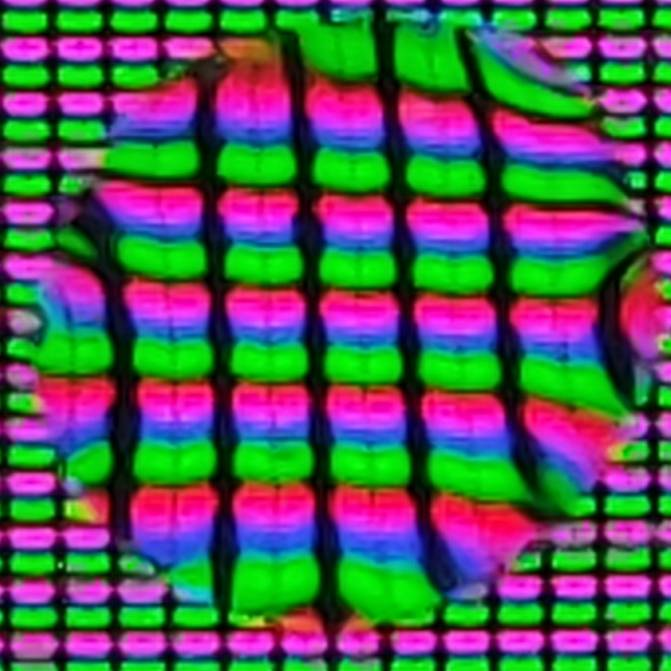
\includegraphics[keepaspectratio,width=150pt]{pixel2.jpg}
    \caption{Color Pixel Pattern of My Laptop}
\end{figure}


\bibliographystyle{ieeetr}
\bibliography{../bib/database}

% \begin{thebibliography}{10}  % 10 is a random guess of the number of total references.
% 	\bibitem{Smith99} Steven W. Smith, ``The Scientist \& Engineer's Guide to Digital Signal Processing", 1999, web: \emph{https://www.analog.com/en/education/education-library/scientist\textunderscore engineers\textunderscore guide.html} 
% \end{thebibliography}

\begin{appendices}
    \section{Code listings}
    \begin{lstlisting}
        // expressionCal.c
        #include<stdio.h>
        #include<math.h>
        int main(){
            char nums[2][4] = {{0},{0}};
            char op[2] = {0};
            char digits[3][2] = {0};
            char ans[6] = {0};
            char buf[6] = {0};
            int pointer = 0;
            int tp = 0;
            int flag = 0;
            printf("Please input your expression: ");
            scanf("%s %s %s",nums[0], op, nums[1]);
            for(int i = 0;i < 2;++i){
                while((nums[i][pointer] != '/')&&(nums[i][pointer])){
                    buf[pointer] = nums[i][pointer];
                    ++pointer;
                }
                if (buf[1])
                    digits[i][0] = (buf[0] - 48) * 10 + buf[1] - 48;
                else if(buf[0])
                    digits[i][0] = buf[0] - 48;
                else
                    digits[i][0] = 1;
                tp = pointer + 1;
                pointer = 0;
                buf[0] = 0;
                buf[1] = 0;
                buf[2] = 0;
                while((nums[i][tp + pointer])){
                    buf[pointer] = nums[i][tp + pointer];
                    ++pointer;
                }
                if (buf[1])
                    digits[i][1] = (buf[0] - 48) * 10 + buf[1] - 48;
                else if(buf[0])
                    digits[i][1] = buf[0] - 48;
                else
                    digits[i][1] = 1;
                pointer = 0;
            }
            if (op[0] == '+'){
                plus(digits[2], digits[0], digits[1]);
                simp(digits[2]);
            }
            else if (op[0] == '-'){
                digits[1][0] *= -1;
                plus(digits[2], digits[0], digits[1]);
                simp(digits[2]);
            }
            else if (op[0] == '*'){
                multi(digits[2], digits[0], digits[1]);
                simp(digits[2]);
            }
            else if (op[0] == '/'){
                char tmp = digits[1][0];
                digits[1][0] = digits[1][1];
                digits[1][1] = tmp;
                multi(digits[2], digits[0], digits[1]);
                simp(digits[2]);
            }
            if (digits[2][0] < 0){
                digits[2][0] *= -1;
                flag = 1;
            }
            if (digits[2][1] != 1){
                if (digits[2][0] > 9){
                    ans[pointer++] = digits[2][0]/10 + 48;
                    ans[pointer++] = digits[2][0]%10 + 48;
                }
                else{
                    ans[pointer++] = digits[2][0] + 48;
                }
                ans[pointer++] = '/';
                if (digits[2][1] > 9){
                    ans[pointer++] = digits[2][1]/10 + 48;
                    ans[pointer++] = digits[2][1]%10 + 48;
                }
                else{
                    ans[pointer++] = digits[2][1] + 48;
                }
            }
            else{
                ans[0] = digits[2][0] + 48;
            }
            if (flag == 0)
                printf("%s %s %s = %s", nums[0], op, nums[1], ans);
            else{
                printf("%s %s %s = -%s", nums[0], op, nums[1], ans);
            }
            return 0;
        }
        void plus(char* c, char* a, char* b){
            c[1] = a[1] * b[1];
            a[0] *= b[1];
            b[0] *= a[1];
            c[0] = a[0] + b[0];
            return;
        }
        void multi(char c[2], char a[2], char b[2]){
            c[1] = a[1] * b[1];
            c[0] = a[0] * b[0];
            return;
        }
        void simp(char c[2]){
            int max = (c[0] > c[1]) ? c[0] : c[1];
            for(int i = 2;i <= sqrt(max); ++i){
                while ((c[0]%i == 0)&&(c[1]%i == 0)){
                    c[0] /= i;
                    c[1] /= i;
                }
            }
            return;
        }
        \end{lstlisting}
    \begin{python}
        # pythonWithSympy.py
        from sympy import simplify
        myexpr = input('Please input your expression: ')
        ans = str(simplify(myexpr))
        print(myexpr + ' = ' + ans)
    \end{python}
    \begin{python}
        #pythonWithoutSympy.py
        string = input(r'Please input your expression: ')
        a, op, b = string.split(' ')
        x = [a, b]
        X = [[], []]
        for i in range(2):
        num = x[i]
        if '/' in num:
        index = num.index('/')
        X[i] = [int(num[:index]), int(num[index + 1:])]
        else:
        X[i] = [int(num), 1]

        if op == '+':
        ans = [X[0][0]*X[1][1] + X[1][0]*X[0][1], X[0][1]*X[1][1]]
        elif op == '-':
        ans = [X[0][0]*X[1][1] - X[1][0]*X[0][1], X[0][1]*X[1][1]]
        elif op == '*':
        ans = [X[0][0]*X[1][0], X[0][1]*X[1][1]]
        elif op == '/':
        ans = [X[0][0]*X[1][1], X[0][1]*X[1][0]]

        for i in range(2,max(ans)):
        while((ans[0]%i == 0) and (ans[1]%i == 0)):
        ans[0] //= i
        ans[1] //= i

        print(string + ' = ' + str(ans[0]) + '/' + str(ans[1]))
    \end{python}
\end{appendices}

\end{document}

